\documentclass{article}

\usepackage[letterpaper,margin=1in]{geometry}
\usepackage[fleqn]{amsmath}
\usepackage{amssymb,amsthm}
\usepackage{graphicx}
\usepackage{algorithm}
\usepackage[noend]{algpseudocode}
\usepackage{xcolor}

\newcommand{\Nrv}   {\operatorname{Nrv}}
\newcommand{\Vrt}   {\operatorname{Vrt}}
\newcommand{\ssx}   {\sigma}
\newcommand{\tsx}   {\tau}
\newcommand{\bdry}  {\partial}
\newcommand{\smplx} {\triangle}
\newcommand{\bigO}  {\operatorname{O}}
\newcommand{\kwd}[1]{{\bf #1}}

\newcommand{\row}[2]{#1[#2,\cdot]}
\newcommand{\col}[2]{#1[\cdot,#2]}

\newtheorem{theorem}            {Theorem}
\newtheorem{corollary}[theorem] {Corollary}
\newtheorem{lemma}[theorem]     {Lemma}
\newtheorem{definition}[theorem]{Definition}
\newtheorem{remark}[theorem]    {Remark}

\newcommand{\Remark}[1]{{\sf [#1]}}
\newcommand{\Warning}[1]{\textcolor{red}{\large [#1]}}


\title{Notes on Distributed Computation of Persistent Homology\\
        using the Blowup Complex}
\author{RHL \and DM}

\begin{document}
\maketitle

\section{Background}

\paragraph{Definitions and Notation.}
The following table outlines the basic notation and terminology.
\vspace{2ex}

\begin{align*}
    && &K                      &   \text{the domain (cell complex)}            \\
    &&n & = |K|           &    \textrm{ complex size} \\
    &&C     &  = \{C_i\}_{i \in \smplx^{p}}      &   \text{cover}                                \\
    &&N &\subseteq 2^{\smplx^{p}}    &                  \text{$\Nrv C$, the nerve of the cover, sub complex of $2^{\smplx^p}$}     \\
    &&K^{\ssx} &= \cap_{i \in \ssx} C_i  & \text{\emph{i do not have a name}}     \\
    &&K^C   & = \cup_{J \subseteq [n]} K^J \times \smplx^J &   \text{the blowup complex}  \\
    &&m & = |K^C_{>0}|    &    \text{ number of blowup cells} \\
    &&m_{\ssx} & = |K^{\ssx}| & \text{  size of thing without a name. }\\
    &&K^C_i & = \{ * \times \ssx \in K^C \mid \dim \ssx = i \} & \text{ $i$-cells of the blowup}             \\
    &&K^C_\sigma & = \{ * \times \ssx \in K^C \} & \text{ cells of the blowup indexed by $\sigma \in N$}             \\
    &&K^C_{<1} & =  K^C_0               &  \text{low dimensional blowup cells}        \\
    &&K^C_{>0} & = K^C - K^C_0               &  \text{high dimensional blowup cells}                               \\
    && & D  \phantom{=}               & \text{graded boundary matrix of the blowup complex}  \\
    && & D_{\ssx}               & \text{submatrix of columns of $D$ whose columns represent the boundaries of $K^C_\sigma$} \\
    && & D^{\tau}_{\sigma} & \text{ submatrix of $D_{\sigma}$ whose rows are indexed by $K^C_{\sigma}$ } \\
    && & D_{>0} & \text{ submatrix of $D$ whose columns are indexed by $K^C_{>0}$ }  \\
    && & D_{<1}  & \textrm{ submatrix of $D$ whose columns are indexed by $K^C_{0}$} \\
    && & D^{\tau}_{>0} & \text{ submatrix of $D_{>0}$ whose rows are indexed by $\tau \in N$}  \\
    && & D^{\tau}_{0} & \text{ submatrix of $D_{0}$ whose rows are indexed by $\tau \in N$} 
\end{align*}

\begin{remark}  
All vertices in $N$ are of the form $\{i\}$ for $i \in [p]$. \\
Let $u,v$ be vertices in $N$. By the definition of $\partial$ for $K^C$ the matrix $D^{u}_{v} = 0$ whenever $u \neq v$. \\
We write $D_i$  and $D^i_{\geq 0}$ for $i \in [p]$ whenever $\{i\} \in N$.
\end{remark}

\section{Algorithm}
\label{sec:algorithm}

\begin{itemize}
    \item $p+1$ processors in total.
    \item Processor $i$ gets matrix $D_i$.
    \item Processor $p$ gets matrix $D_{>0}$,
          with columns indexed by $K^C_{>0}$ and rows indexed by $K^C$.
\end{itemize}

\subsection{Version 1}
\begin{enumerate}
    \item
        Each processor $i \in \{ 0 \ldots p-1 \}$:
        \begin{itemize}
            \item Reduce        $D_i \to R_i$.
            \item Row-reduce    $R_i = S_i P_i$,
                where $P_i$ is (almost) a permutation matrix,
                and   $S_i$ is upper-triangular. Compute $S_i^{-1}$ while at it.
                See Algorithm~\ref{alg:row-reduce}.
        \end{itemize}
    \item
        Processor $p$:
        \begin{itemize}
            \item Reduce $D_{>0} \to R_{>0}$, see Figure~\ref{fig:matrices} on
                  the left.
            \item Send $R^i_{>0}$ to processor $i$.
                $R^i_{>0}$ is the subset of $R_{>0}$
                where the rows are indexed by $K^C_i$.
        \end{itemize}
    \item
        Processor $i$:
        \begin{itemize}
            \item Compute $Q^i_{>0} = S^{-1}_i \cdot R^i_{>0}$.
            \item Send $Q^i_{>0}$ and $P^i$ back to processor $p$.
        \end{itemize}
    \item
        Processor $p$:
        \begin{itemize}
            \item
                Concatenate matrices $Q^i_{>0}$, together with the remainder of
                $R_{>0}$ (the part where the rows are indexed by $K^C_{>0}$),
                together with matrices $P_i$.
                Put all the columns and rows in the correct (filtration) order.
                Call the resulting matrix $T$, see Figure~\ref{fig:matrices} on
                the right.
            \item Reduce $T$ using the cascade. Its lowest ones are the answer.
        \end{itemize}
\end{enumerate}

\begin{figure}
    \centering
    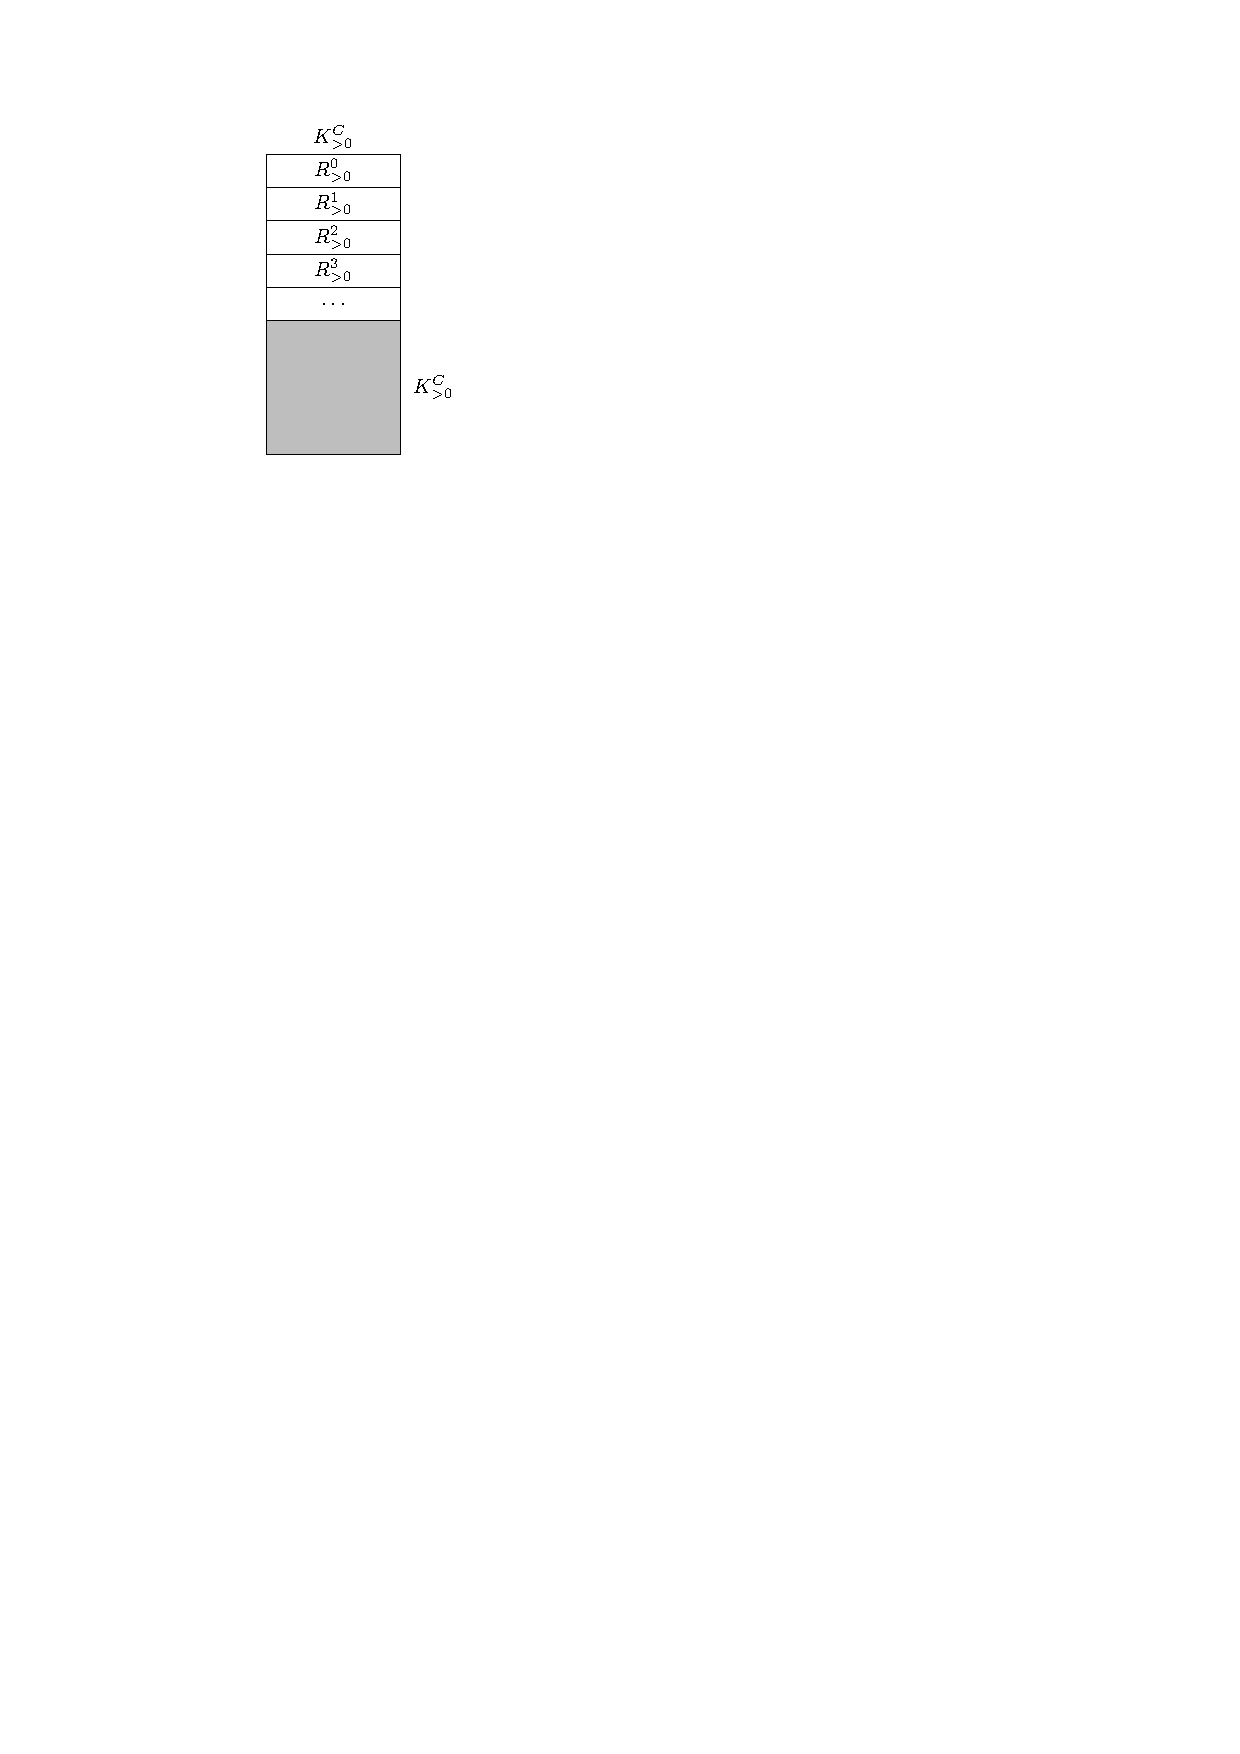
\includegraphics{figs/matrix-Rg0}
    \hspace{1in}
    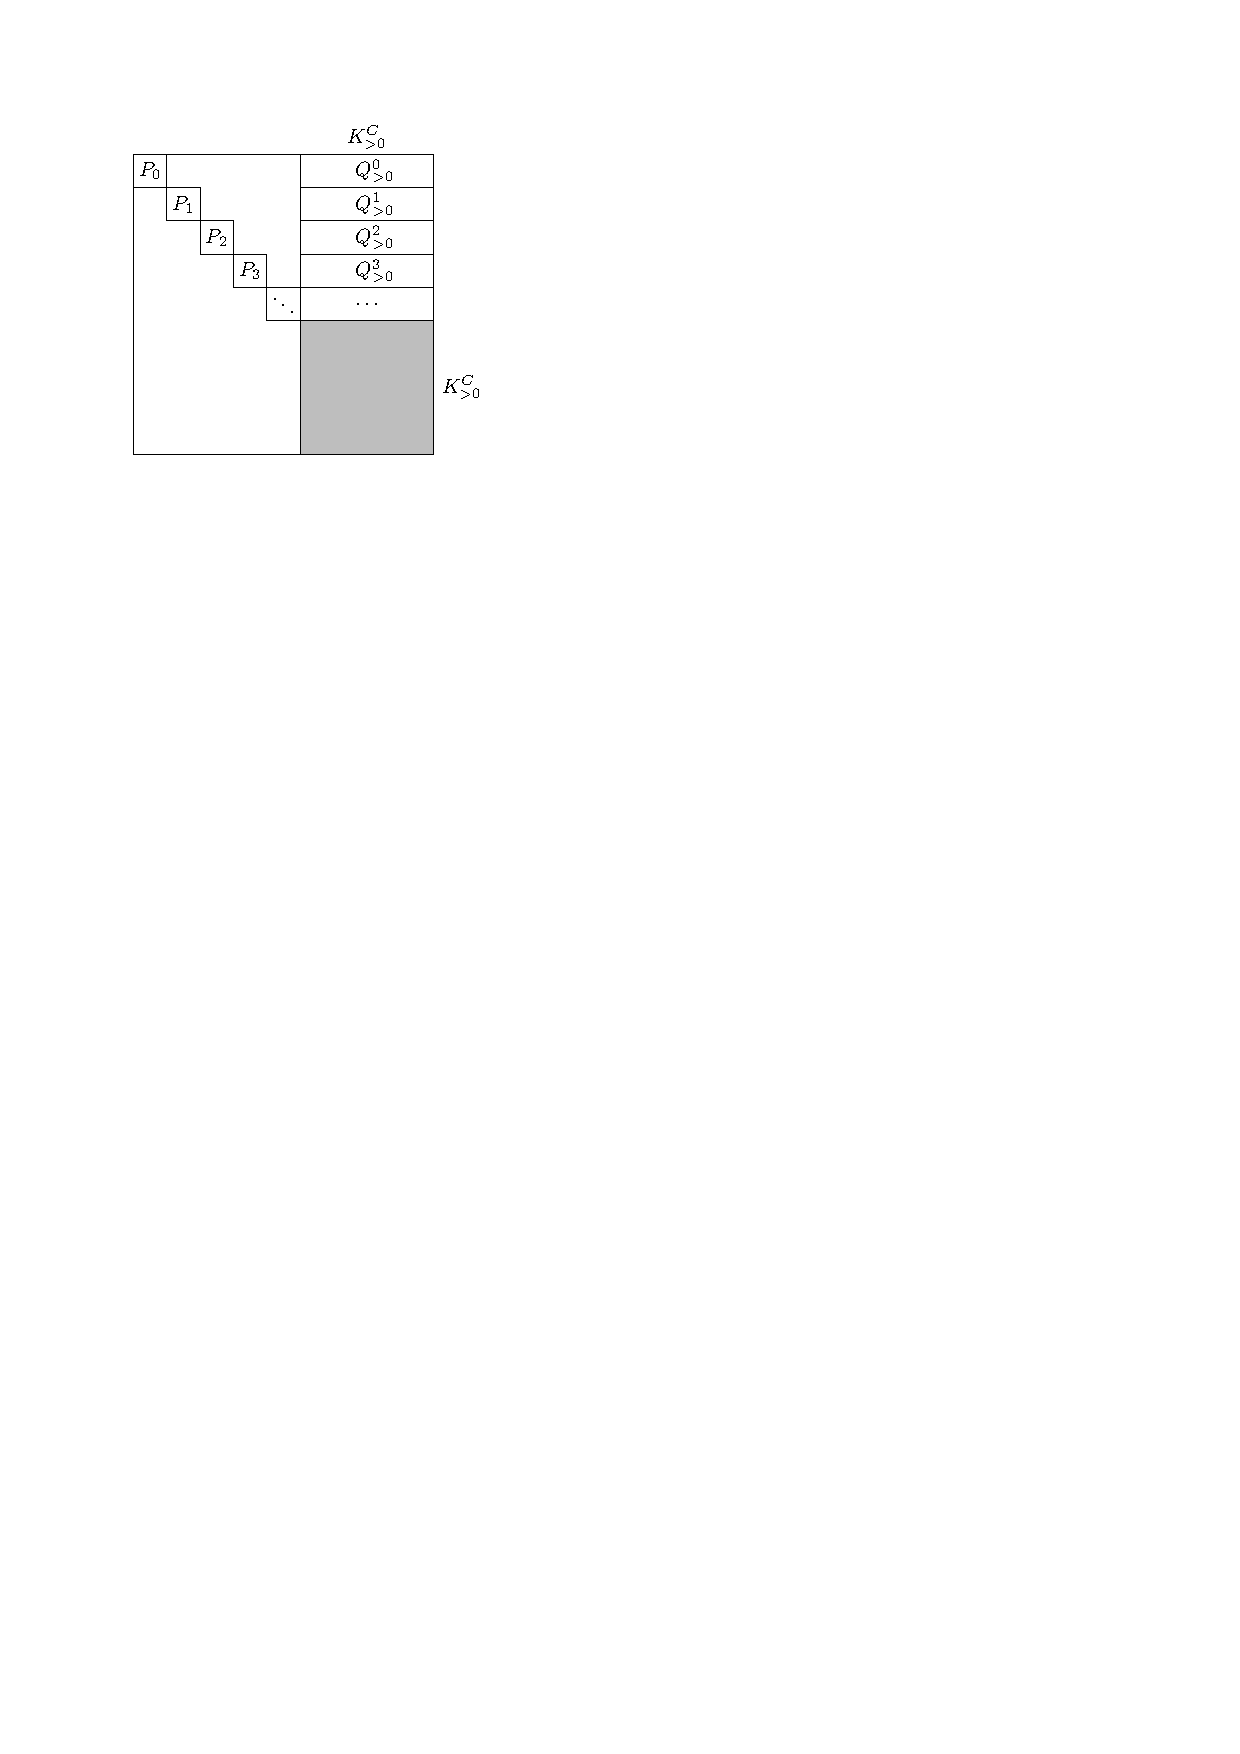
\includegraphics{figs/matrix-T}
    \caption{Structure of matrices $R_{>0}$ (left) and $T$ (right).
             The columns and rows of $T$ need to be put into the filtration order.}
    \label{fig:matrices}
\end{figure}


\subsection{Version 2}

We assume that each processor knows not only its local region of the domain, but also
which cover sets intersect it and where. In matrix terms, it knows both matrix
$D_i$ and $D^i_{>0}$.

\begin{enumerate}
    \item
        Each processor $i \in \{ 0 \ldots p-1 \}$:
        \begin{itemize}
            \item Reduce        $D_i \to R_i$.
            \item Row-reduce    $R_i = S_i P_i$.
                  See Algorithm~\ref{alg:row-reduce}.
            \item Compute       $\bar{Q}^i_{>0} = S^{-1}_i \cdot D^i_{>0}$.
                \begin{remark}
                    Naturally, one wouldn't explicitly compute $S_i$ or
                    $S^{-1}_i$, but rather apply the same row operations to
                    $D^i_{>0}$ as are being performed on $R_i$ to obtain $P_i$. \\
                \end{remark}
            \item Send $\bar{Q}^i_{>0}$ and $P_i$ to processor $p$.
        \end{itemize}

    \item
        Processor $p$:
        \begin{itemize}
            \item
                Concatenate matrices $\bar{Q}^i_{>0}$, together with the remainder of
                $R_{>0}$ (the part where the rows are indexed by $K^C_{>0}$),
                together with matrices $P_i$.
                Put all the columns and rows in the correct (filtration) order.
                Call the resulting matrix $T$, see Figure~\ref{fig:matrices} on
                the right.
            \item Reduce $T$ using the cascade. Its lowest ones are the answer.
        \end{itemize}
\end{enumerate}

\subsection{Analysis}

\begin{theorem}
    Lowest ones of the reduced $T$ give the correct pairing.
\end{theorem}

\begin{theorem}
    $|T| = (n-m) + nm$. $T$ can be reduced using the cascade
    (Algorithm~\ref{alg:cascade}) in time $\bigO(n m^2)$,
    while keeping its size $\bigO(nm)$.
\end{theorem}

\begin{remark}
    In both versions of the algorithm, there is an obvious optimization.
    When processor $i$ sends to processor $p$ matrix $P_i$, it suffices to send
    only those elements that fall in rows with non-zero entries in matrix $Q^i_{>0}$.
    It's an open question how effective this optimization is in practice.
    \textbf{Ryan:} This seems like it will be easy to implement, one way or the other.
\end{remark}

\begin{remark}
    As usual with the blowup complex, if dimension of $K$ is $d$, we never need
    to construct higher than $(d+1)$-skeleton of the blowup complex, since it
    captures all the homology that can possibly exist.
\end{remark}

\section{Matrix Algorithms}

\Remark{Need to change 1s to the actual coefficients.}
\begin{algorithm}
    \begin{algorithmic}
        \State $P = R, S = I, S^{-1} = I$
        \ForAll{rows $i$ of $P$, from the bottom up}
            \If{no lowest one in row $i$}
                \State \kwd{continue}
            \EndIf
            \State $j = $ the column of the lowest one in row $i$
            \ForAll{non-zero entries $P[i',j]$ in column $\col{P}{j}$}
                \State{subtract row $\row{P}{i}$ from row $\row{P}{i'}$
                       (really zero out the entry $P[i',j]$)}
                \State{add column $\col{S}{i'}$ to column $\col{S}{i}$ (left to right)}
                \State{subtract row $\row{S^{-1}}{i}$ from row $\row{S^{-1}}{i'}$}
            \EndFor
        \EndFor
    \end{algorithmic}
    \caption{Row reduce: $R = SP$, $P = S^{-1} R$.}
    \label{alg:row-reduce}
\end{algorithm}

\section{Cascade}

\begin{definition}
    A matrix $T$ is said to be an \emph{almost-permutation matrix} if all but
    $k$ of its columns have at most one non-zero entry and such entries do not
    collide (i.e., they appear in unique rows).
    We call the columns with at most one non-zero entry \emph{ultra-sparse}.
\end{definition}
%
Figure~\ref{fig:almost-permutation} illustrates an almost permutation matrix.
%
Matrix $T$ in Section~\ref{sec:algorithm} is an almost-permutation matrix with $k = m$.
(Concatenation of matrices $P_i$ gives the columns with unique, non-colliding
non-zero entries.)
%
\begin{figure}
    \centering
    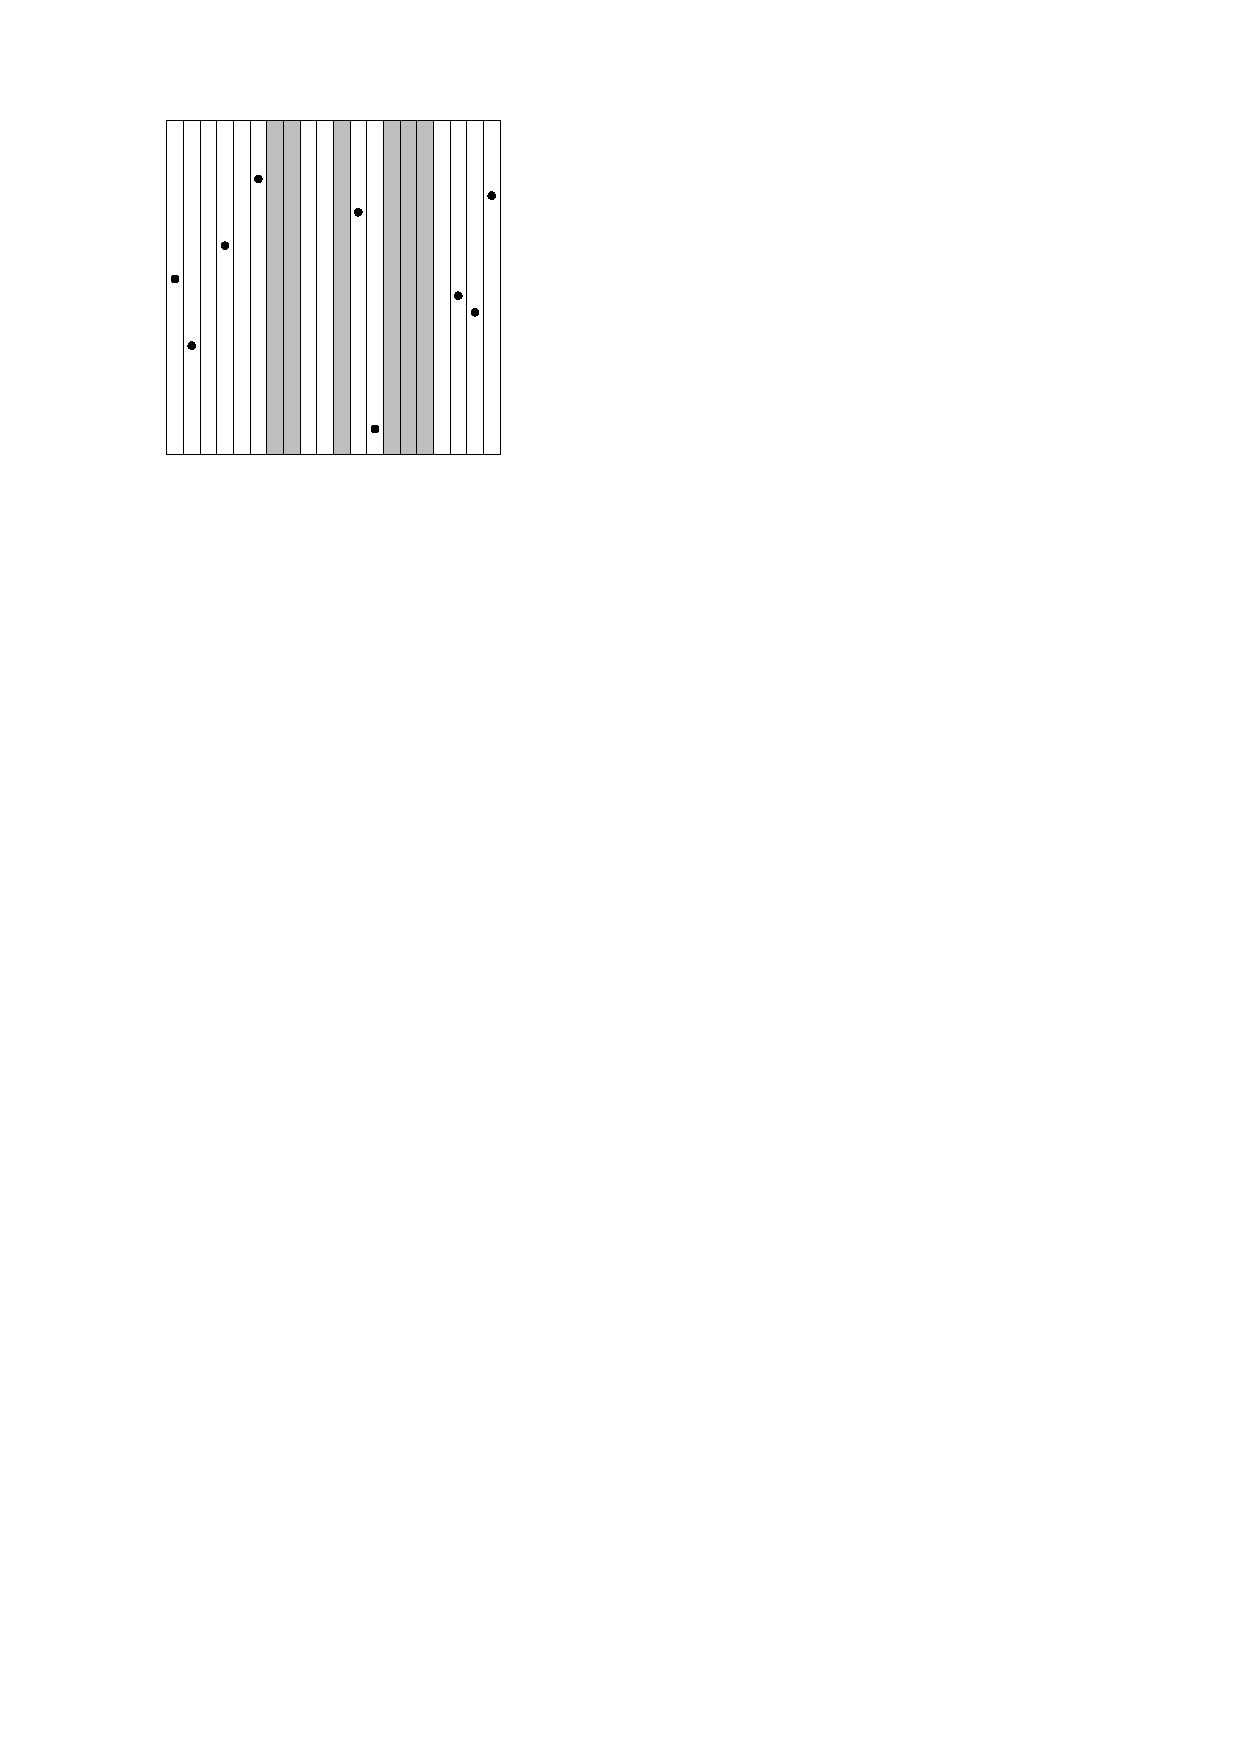
\includegraphics{figs/almost-permutation}
    \caption{An almost-permutation matrix $T$, with $k = 9$ ultra-sparse columns.
             Grey columns may contain any number of non-zero elements. The white
             columns contain at most one non-zero element, and all such elements
             appear in unique rows.}
    \label{fig:almost-permutation}
\end{figure}
%
Algorithm~\ref{alg:cascade} efficiently reduces an almost-permutation matrix.
%
\begin{algorithm}
\begin{algorithmic}
    \ForAll{columns $\col{T}{j}$, from left to right}
        \State \kwd{if} $\col{T}{j} = 0$, \kwd{continue}
        \State $i$ = row of the lowest non-zero entry in $\col{T}{j}$
        \If{$\col{T}{j}$ is an ultra-sparse non-zero column}
            \If{$i$ collides with a non-ultra-sparse column $\col{T}{j'}$}
                \State swap columns $\col{T}{j}$ and $\col{T}{j'}$
                \State subtract $\col{T}{j'}$ from $\col{T}{j}$, i.e., zero out $T[i,j]$
            \Else
                \State Nothing to do: ultra-sparse columns cannot collide.
            \EndIf
        \EndIf
        \If{$T[i,j]$ has a collision with a column $j' < j$}
            \State subtract $\col{T}{j'}$ from $\col{T}{j}$. Equivalently, zero out $T[i,j]$
        \EndIf
    \EndFor
\end{algorithmic}
\caption{Cascade algorithm for reduction of an almost-permutation matrix $T$.}
\label{alg:cascade}
\end{algorithm}

Algorithm~\ref{alg:cascade-row} recasts Algorithm~\ref{alg:cascade} in the row
form.
%
The last two lines of Algorithm~\ref{alg:cascade-row} are equivalent to
first swapping columns $j$ and $j'$ and then subtracting the new column $j$ from
the new column $j'$. (Up to coefficients, as the rest of this write-up.)
The salient point is that after these last two lines, we never need column
$\col{T}{j}$ again, except for the location of its lowest non-zero entry, so we
can zero it out.

\begin{algorithm}
\begin{algorithmic}
    \ForAll{rows $\row{T}{i}$, from bottom up}
        \State $J$ = the sequence of columns with the lowest non-zero entry in $\row{T}{i}$.
        \State $j$ = the first entry in $J$
        \If{$\col{T}{j}$ is ultra-sparse}
            \ForAll{$j' \in J, j' > j$}
                \State subtract $\col{T}{j}$ from $\col{T}{j'}$
            \EndFor
        \Else
            \ForAll{$j' \in J, j' > j$ and $\col{T}{j'}$ not ultra-sparse}
                \State subtract $\col{T}{j}$ from $\col{T}{j'}$
            \EndFor
            $j'$ = the first ultra-sparse column in $J$
            \ForAll{$j'' \in J, j'' > j'$ and $\col{T}{j''}$ ultra-sparse}
                \State subtract $\col{T}{j'}$ from $\col{T}{j''}$
            \EndFor
            \State subtract $\col{T}{j}$ from $\col{T}{j'}$
            \State zero out all but the lowest entry of $\col{T}{j}$
        \EndIf
    \EndFor
\end{algorithmic}
\caption{The row form of the cascade algorithm for reduction of an almost-permutation matrix $T$.}
\label{alg:cascade-row}
\end{algorithm}



\begin{theorem}
    \label{thm:cascade-analysis}
    Algorithm~\ref{alg:cascade} reduces an $n \times n$ almost-permutation
    matrix with $k$ ultra-sparse columns in time $\bigO(nk^2)$ using $\bigO(nk)$
    space.
\end{theorem}


\section{Pairwise Intersections Do Not Suffice}

Figure~\ref{fig:triple-intersection} illustrates a triple intersection. We
assume that extending the space outside the figure, the cells form a 2-cycle.
This 2-cycle has to use the triangle $u \times t$ in the blowup complex.

\begin{figure}
    \centering
    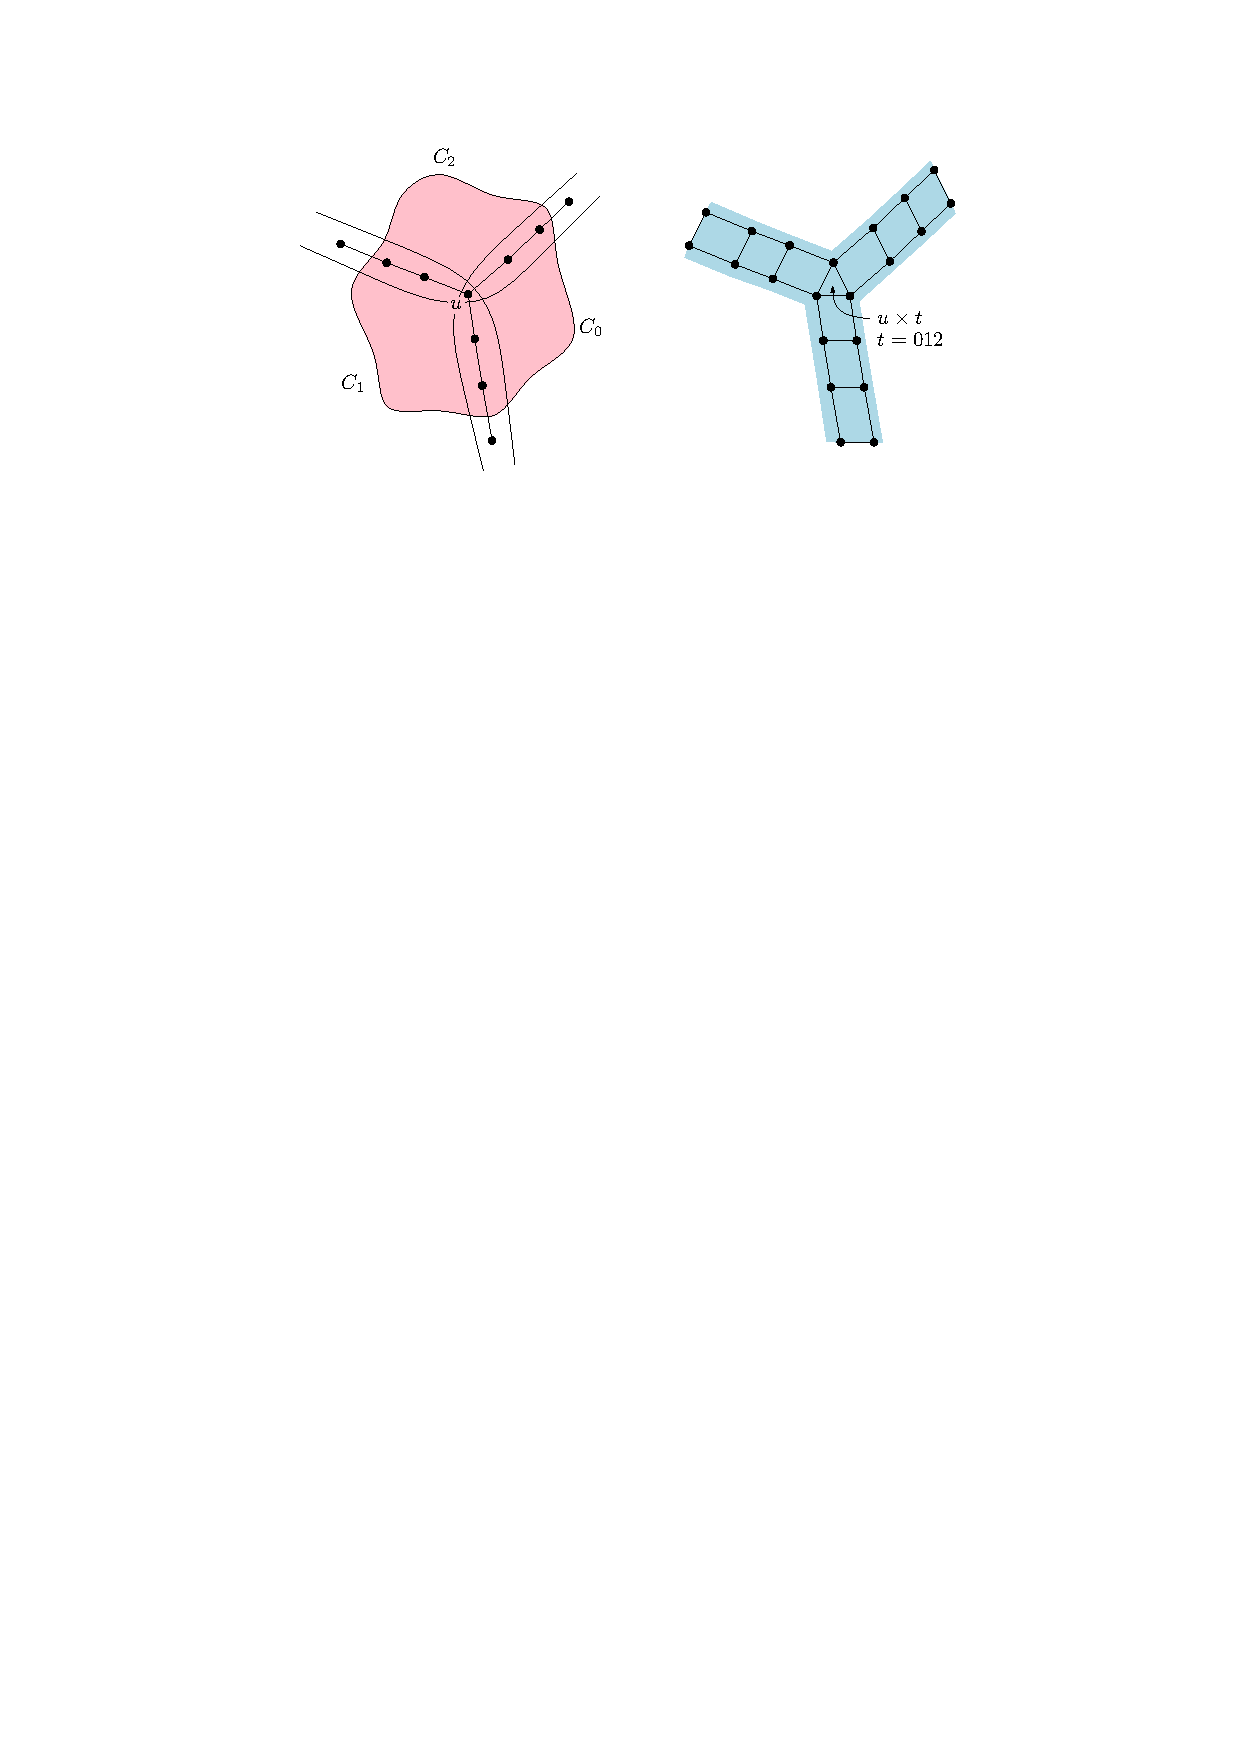
\includegraphics{figs/triple-intersection}
    \caption{The 2-cycle cannot be formed without $u \times t$.}
    \label{fig:triple-intersection}
\end{figure}


\paragraph{Correct, but incomplete argument.}

The cells of the blowup complex $\{ \ssx_i \times \Delta_j \}_{i,j}$ are ordered
lexicographically, where the first order (of cells $\ssx_i \in K$) is given by
the original filtration, and the second order by sorting all the faces of
simplex $\Delta_j$ by dimension.
Figure~\ref{fig:blowup-cell} illustrates the structure of the reduced boundary
matrix for a block $\ssx \times \Delta$, where $\Delta$ is a triangle.

\begin{figure}
    \centering
    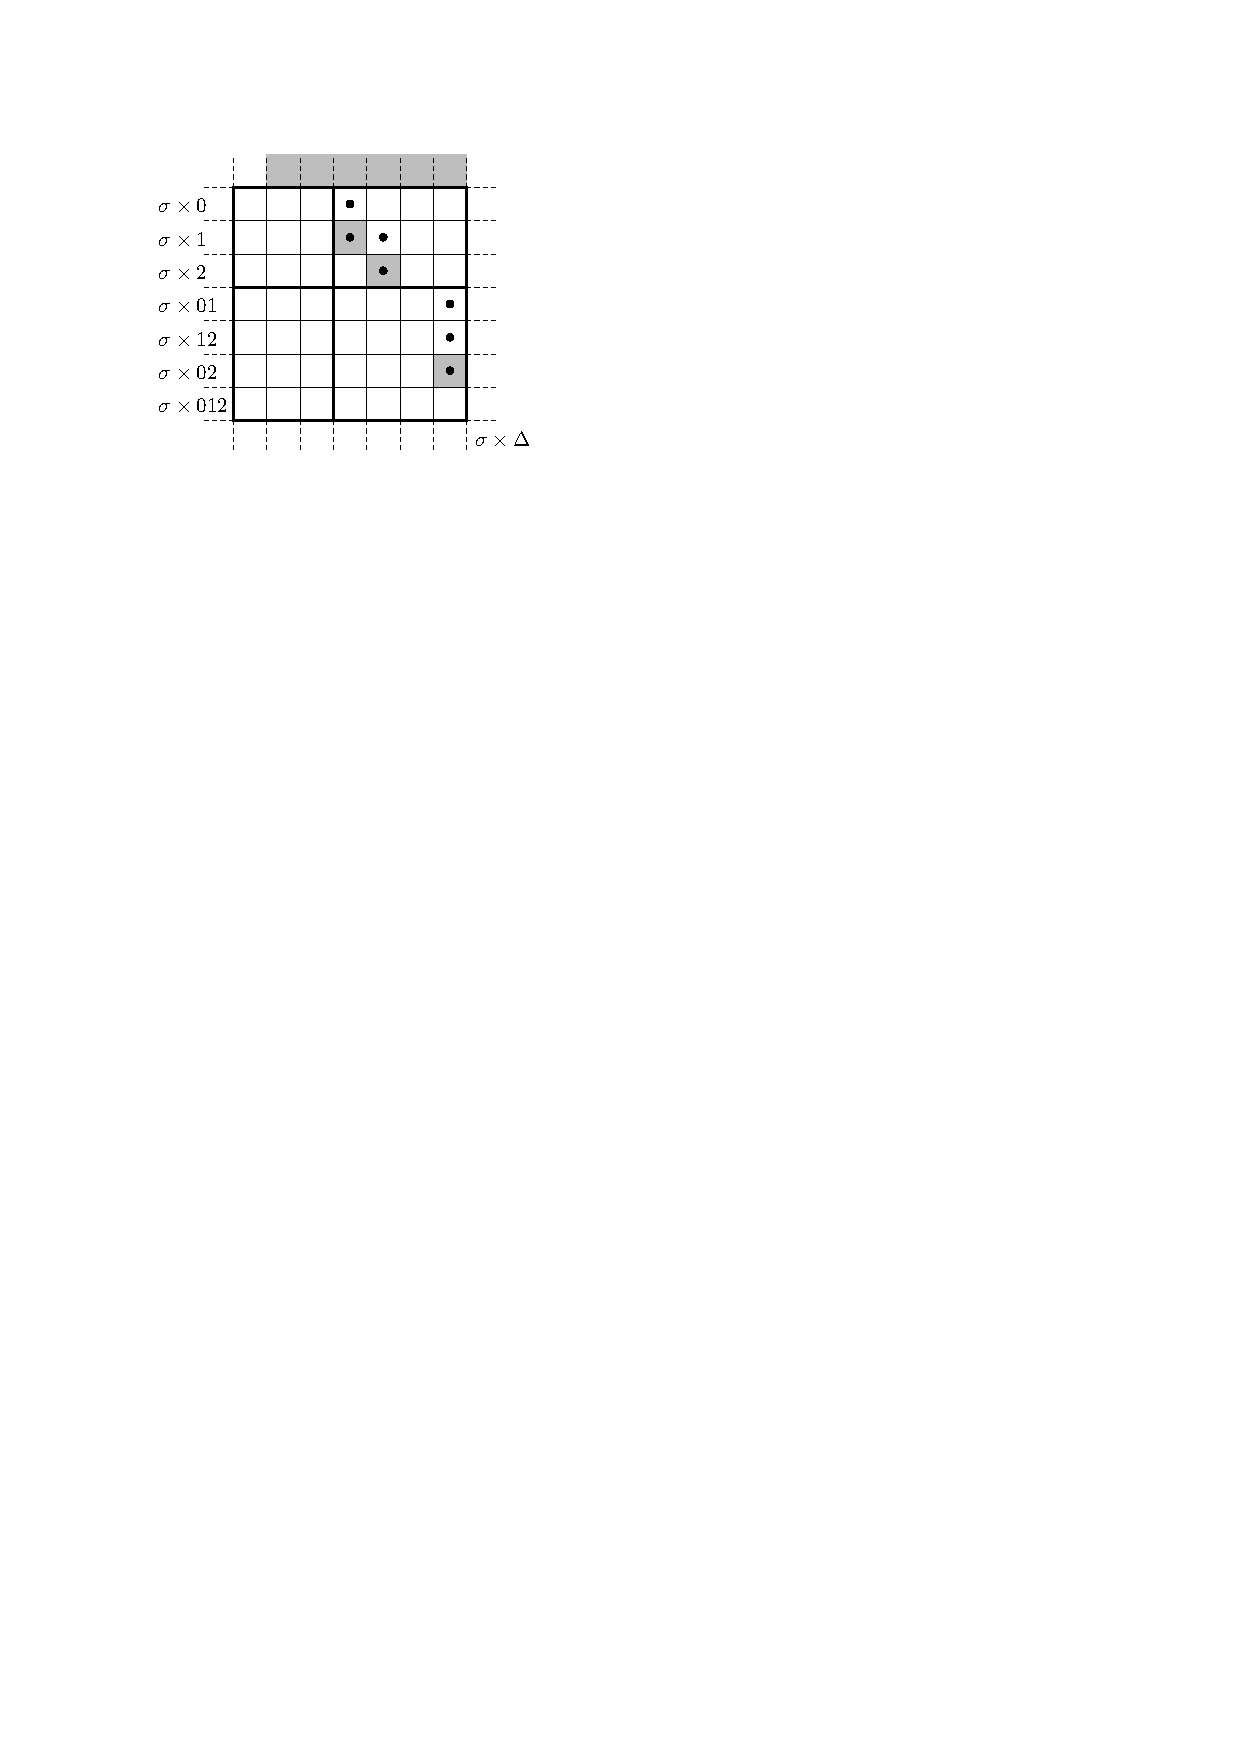
\includegraphics{figs/blowup-cell}
    \caption{The structure of pairings in a blowup of a single cell $\ssx$ that
             appears in the intersections of three cover sets $C_0, C_1, C_2$.}
    \label{fig:blowup-cell}
\end{figure}

Since $\Delta$ is a simplex, it is collapsible. Therefore, its homology is
trivial. So half of the cells in the block will kill the other half of
the cells in the block. (Restricted to the block the reduction is just that of a
simplex. Since a negative cell can only get paired with a positive cell, the
other half of the cells are positive \emph{in the entire blowup complex}, and
therefore their columns are zero.)
%
\Remark{It would be nice to understand directly why the column of
$\ssx \times \alpha$, where $\alpha$ is a positive simplex in the filtration of
$\Delta$, is zero in the entire blowup complex. I.e., what exactly happens to
them outside the block.} 
%\Warning{This argument is incorrect!}
%%
%The only cells outside the block that have a cell $\ssx \times \alpha$ in their
%boundary, with $\dim \alpha > 0$, are cells of the form $\tsx \times \alpha$,
%with $\ssx \in \bdry \tsx$.
%But those cells are paired within their own block, and, therefore, never need a
%column from the block of $\ssx \times \Delta$. It follows that we can discard
%all the columns $\ssx \times \alpha$ with $\dim \alpha > 1$ and all the rows
%$\ssx \times \alphaa$ with $\dim \alpha > 0$.

%\begin{remark}
%    In fact, it suffices to keep a spanning forest of the edges in $\Delta$ and
%    discard the rest of its faces. This way we'll get exactly the correct
%    persistence, with no extra zero columns sitting around.
%    \emph{There's got to be an algebraic way to see this.}
%\end{remark}

\section{Some commutative algebra for distributed memory filtrations}
Given a basis for the finitely generated $k[t]$ module define the 
\emph{critical grade} of a basis element $\sigma$, denoted 
$\operatorname{critical-gr}(\sigma)$ to be it's grade.

Suppose $M$ is the chain $k[t]$-module of our base space and $N$ is the 
$k[t]$-module for the nerve. Initially, the filtration on the nerve is skeletal. 
The blowup complex $B$ is again a $k[t]$-module and it's basis is prescribed by 
an elementary tensor $\sigma \otimes \tau$ for $\sigma$ in the basis of $M$ and 
$\tau$ in the basis for $N$. The filtration on the blowup complex prescribes 
that 
$\operatorname{critical-gr}(\sigma \otimes \tau) = \operatorname{critical-gr}(\sigma)$. 
The prescribed filtration on the blowup complex also refines the filtration on 
the nerve. Namely,
\[  \operatorname{critical-gr}(\tau) = \min_{\substack{\sigma \in M \\ N(\sigma) = \tau}} \operatorname{critical-gr}(\sigma) \]
We need not respect this refined grade, but, it is 
useful for a coarse view of communication between the machines.

Since we suppose that each processor knows the grade on each cell $\sigma$ it 
has in the input, we know the grade of each cell of the blowup complex at 
construction.  By storing this grade with each cell we may use this to aid in 
the distributed filtration. Comparing two cells may be achieved by first 
comparing grades, then comparing product cells of the same grade in any 
dimension preserving manner. For example, assuming that the input filtration is 
a total order, then comparisons within the same grade amount to ordering based 
on the nerve. If all the elements happen to live in the same grade, we get 
precisely the filtration given in Lewis \& Zomorodian. 
\section{}
There are a number of tasks that may be carried out independently, 
I see three major groups of tasks, i'll call them stage 0, stage 1 and stage 2. 
Here is stage 0:
1)  reduce each piece of the disjoint union rel the subcomplex corresponding to 
the intersection,
2)  taking the maximal cells of the nerve, we may reduce their realization as a 
complex once, and then glue this into the cells of the blowup complex of higher 
nerve dimension.
3) within each piece of the disjoint union, we may now reduce the subcomplex 
which we rel'd out by in (1), taking care to first zero out columns which we 
know are positive from (2). 

The union of all these column chunks form the entire (partially reduced) blown 
up boundary matrix.  It seems that the explicit zeroing which we can perform in 
Stage 0, will save considerable work from what we were going to by just reducing 
each piece of the disjoint union. 

Stage 1 of course amounts to taking these columns sticking them in the correct 
column/row order and then reducing again. Observe that while this is a chunking 
type procedure, we have more structure here. In particular, 
the nerve hopefully has some interesting topology. 
In stage 1 we do the following things:

4) we reveal the remainder of these intersections subcomplexes 
(now including blowup cells of high nerve-d) , to the disjoint union.
5) we reduce these intersections against the disjoint union

At this point we have on each machine a number of relative cycles and boundaries. 
It should be clear that aside from the trivial pairings we found, some of the 
pairings from step (1) are actual pairs. In particular, pairs which were killed 
before the grade at which an intersection appeared are certainly real features. 
A pairing which lives in a grade *after* the first intersection however still 
may not be a true pairing. 

Observe that up until now we have not done any real communication. 
This is of course Stage 2. More writing soon.


\end{document}
